\documentclass{article}

\usepackage{amsmath}
\usepackage{graphicx}
\usepackage[colorlinks=true]{hyperref}

\title{MP1 \\ CS 598: Parallel Migratable Objects}
\author{Fall 2013}
\date{Due date: Thursday, September 26, 10pm}

\begin{document}
\maketitle

\textbf{Description:} 
For this assignment you need to write a Charm++ program which does manual load
balancing of integer numbers among elements of a 1D chare array using the 
given parallel prefix code in the class slides or with your own parallel 
prefix code. 

First, you create a chare array of size $s$, where each chare $i$ generates 
(and hence owns) $n_i$ integer numbers. For every chare $i$, $n_i$ is a 
randomly generated number between $min$ and $max$. 
$min$, $max$ and $s$ are command line parameters. 
Once $n_i$ is generated, chare $i$ generates $n_i$ random 
integers (using rand()). The task is to load balance the count
of integer number among chares, i.e. if $n = n_1 + n_2 \cdots n_s$,
each chare should get approximately $\frac{n}{s}$ integers.

You can either use Quiescence Detection (with CkStartQD(..) function, for more
information about QD go to related
\href{http://charm.cs.illinois.edu/manuals/html/charm++/12.html#SECTION02350000000000000000}{manual
section}) to terminate or your own method to detect when
the load balancing is complete. \\

\emph{Correctness Test}: The checksum of the integers in the beginning
should be same as checksum of the integers after the load balancing
Use \emph{bitvec\_or} operation of the integers to compute checksum in Charm++
reduction. \\

\emph{Hint}: Use reduction to get the average number of integer per chare. 
The average should be useful in deciding which integers should be at which chares
after load balancing. Use exclusive parallel prefix (count of integers in chare $i$
is not counted in $prefix_i $) to decide which chare array element 
should send which integers to which chare array element. Figure~\ref{prefix}
may provide further hints. \\

\begin{figure}[h]
\centering
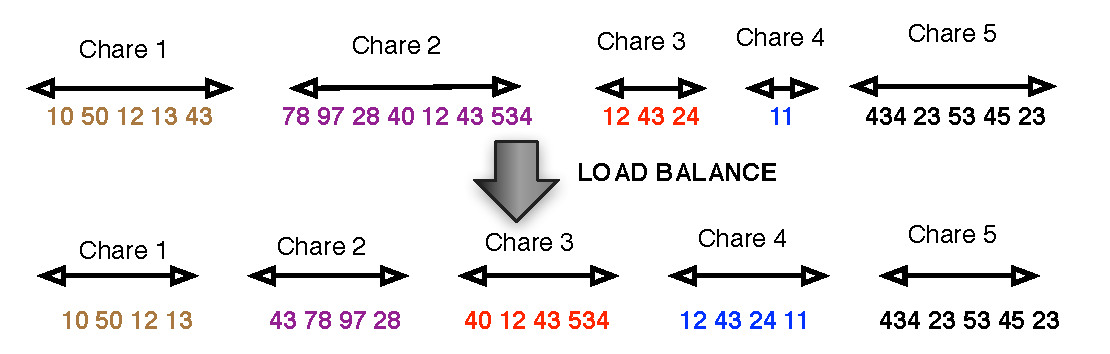
\includegraphics[width=\textwidth]{prob1.pdf}
\caption{Load balancing integers among chares.}
\label{prefix}
\end{figure}

\textbf{Running your code:}
The program should have the following signature: \\
\textit{./charmrun ./mp1 +p4 chare-array-size min max} \\

You should test your code on Taub cluster up to 64 nodes. You can start with a small
number of processors and once you make sure your algorithm works, you can test
with more number of processors. You can use 1024 as
\textit{chare-array-size} and \textit{min/max} could be in the range of [5,000 - 30,000].
\\ \\ \\

\textbf{Submission:}
Create an mp1 directory in your SVN repository folder and add your code into
that folder and check in the your code.
\begin{itemize}
\item  For each file F you create, that you want to check in, do: \\
        \textit{svn add F}\\
        and frequently (after you have modified F, and have the next better
        version) do:\\ 
        \textit{svn ci F}
\item  There will be a penalty for late submissions.
\end{itemize}

\end{document}
